%=============================================================================
% Thesis Template in LaTex
%
% File:  Kostenstruktur -- Fallstudie
% Author(s): Jürgen Hackl <hackl@ibi.baug.ethz.ch>
%            Clemens Kielhauser <kielhauser@ibi.baug.ethz.ch>
%
% Creation:  27 Jan 2014
% Time-stamp: <Tue 2013-08-13 20:14 juergen>
%
% Copyright (c) 2014 Infrastructure Management Group (IMG)
%               http://ibi.ethz.ch
%
% More information on LaTeX: http://www.latex-project.org/
%=============================================================================

% Unterkapitel Kostenstruktur
% ---------



\subsection*{Wartungskosten}
\label{sub:Unterhalt}

Die Berechnung der Wartungskosten $K_{W}$ der Infrastruktur erfolgt gemäss der Formel \ref{eq.2}. Sie setzen sich zusammen aus den einmaligen Investitionskosten für den Bau der Infrastruktur $K_{Bau}$ und den jährlich anfallenden Wartungskosten $K_{Wartung,t}$.

\begin{equation}
K_{W} = K_{Bau} + \sum_{t=0}^T \  K_{Wartung,t}  \label{eq.2} \\ 
\end{equation}


{\setstretch{0.6}
wobei:
\begin{conditions}
 K_{W}      	     			&  Totale Wartungskosten für $T$ Jahre  \\
 K_{Bau}           			    &  Baukosten der Variante     \\
 K_{Wartung,t}                  &  Wartungskosten pro Jahr     
\end{conditions}
}


Die Berechnung der jährlichen Wartungskosten erfolgt anhand Formel \ref{eq.3}. Die angenommenen Einheitskosten für den Bau und die Instandhaltung sind anhand von Werten der Fachliteratur hergeleitet und werden nachfolgend erläutert. 

\begin{equation}
K_{Wartung,t} = \sum_{k=1}^2 \ EK_{Wartung,k} \cdot s_{k} \cdot b_{k}  \label{eq.3} 
\end{equation}

{\setstretch{0.6}
\begin{align*}
	  k &=
      \begin{cases}
        \begin{aligned}
          & 1 \\
          & 2
        \end{aligned} &
        \begin{aligned}
         & \text{für}\ \thinspace \\
         & \text{für}\ \thinspace
        \end{aligned}
        \begin{aligned}
          & \text{Strasse} \\
          & \text{Unterführung}
        \end{aligned}
      \end{cases} \\
\end{align*}

wobei:
\begin{conditions}
 EK_{Wartung,k}      	     	&  Einheitskosten pro [$m^2$]   \\
 s_k	    	     			&  Länge der Infrastruktur in [$m$] \\
 b_k	    	     			&  Breite der Infrastruktur in [$m$]   \\
 k								&  Art der Infrastruktur  
\end{conditions}
}

Die Erstellung zweier neuer Radstreifen à je 1.5 $m$ Breite kostet pro Laufmeter 850 CHF. Die Investitionskosten pro Quadratmeter für den Bau einer Velounterführung unter dem Lastfall Eisenbahn, betragen 3750 CHF. Der Bau der Zufahrtsrampen zu den Velounterführungen kostet pro Rampe 130'000 $CHF$. \\
Die Wartungskosten welche für die Instandhaltung der Strassen, inklusive der Fahrradstreifen und der Fussgängerwege anfallen, betragen jährlich 5 \thinspace $\frac{CHF}{m^2}$. Die wartungsintensivere Infrastruktur der Unterführung wird jährlich mit 30 \thinspace $\frac{CHF}{m^2}$ instand gehalten. (\cite{Baukosten2010}) 

Diese Kosten sind hauptsächlich von der Auslastung der Infrastruktur und vom Gewicht der Fahrzeuge, die sie befahren, abhängig. Da diese Kosten im Vergleich zu den anderen Kostenpositionen deutlich geringen ausfallen, verzichte ich auf eine Variation dieser Parameter über den betrachteten Zeitraum. Die nachfolgende Tabelle \ref{tab:t-04-03-01-Unterhalt} fasst die für die Besitzer anfallenden Einheitskosten zusammen.

%=============================================================================
% Thesis Template in LaTex
%
% File:  t-05-01-IsingModel.tex -- Table for the Ising
% Author(s): Juergen Hackl <hackl@ibi.baug.ethz.ch>
%            Clemens Kielhauser <kielhauser@ibi.baug.ethz.ch>
%
% Creation:  27 Jan 2014
% Time-stamp: <Tue 2013-08-13 20:14 juergen>
%
% Copyright (c) 2014 Infrastructure Management Group (IMG)
%               http://ibi.ethz.ch
%
% More information on LaTeX: http://www.latex-project.org/
%=============================================================================

\begin{table}[h!]
\flushleft
%\center
\renewcommand{\arraystretch}{1.4}
%\captionsetup{justification=centering}

\begin{tabular}{ @{} lc|ccc @{} }
                 &                         & Fahrbahn  & Veloweg  & Unterführung \\ \hline
Wartungskosten &$\frac{CHF}{m^2 \ Jahr}$ &     5     &     5    &      30        \\
Baukosten        &$\frac{CHF}{m}$ 		   &     -     &   850    &     18'900        
\end{tabular}
\caption{Bau- und Wartungskosten}
\label{tab:t-04-03-01-Unterhalt}
\end{table}

%\begin{table}[h!]
%\flushleft
%\renewcommand{\arraystretch}{1.4}
%\small\renewcommand{\arraystretch}{1.2} 
%
%
%\begin{tabular}{@{}p{3.3cm} p{4cm} p{1cm} r l @{}} \\   
%\toprule
%\textbf{Interessensgruppe} & \textbf{Kostentyp} & \textbf{Symbol} & \multicolumn{2}{c}{\textbf{Einheitskosten}} 			\\
%\midrule

%\bottomrule

%\end{tabular}

%\end{table}


%=============================================================================
% EOF
%

%%% Local Variables:
%%% mode: latex
%%% TeX-master: "../guidelines"
%%% End:



\newpage

\subsection*{Betriebskosten}
\label{sub:Betrieb}

Die Fahrzeugbetriebskosten $K_{B}$ sind als die, jährlich für den Nutzer für die Instandsetzung und den Betrieb eines Fahrzeugs anfallenden Kosten definiert und somit die Kosten die bei der Nutzung der Infrastruktur entstehen können. \\
Die Kosten, die für den betrachteten Zeitraum von $T$ Jahren anfallen, werden gemäss Formel \ref{eq.6} durch die Multiplikation der Anzahl Nutzer mit der zurückgelegten Distanz und mit den Einheitskosten pro Fahrzeugkilometer, berechnet. 

\begin{equation}
K_{B} =  \sum_{t=0}^T \Biggl[ \sum_{j=1}^2 \ EK_{B,j} \cdot s_{j} \cdot DTV_{j,t} \Biggr] \cdot 365  \label{eq.6} \\
\end{equation}

{\setstretch{0.6}
\begin{align*}
	 j &=
      \begin{cases}
        \begin{aligned}
          & 1 \\
          & 2
        \end{aligned} &
        \begin{aligned}
         & \text{für}\ \thinspace \\
         & \text{für}\ \thinspace
        \end{aligned}
        \begin{aligned}
          & MIV \\
          & Velo
        \end{aligned}
      \end{cases} \\
\end{align*}

wobei:
\begin{conditions}
 K_{B}			   &  Totale Fahrzeugbetriebskosten \\
 EK_{B,j}	       &  Einheitskosten pro [$km$] \\
 s_j	    	   &  Länge der Infrastruktur; nach Fahrzeugtyp in [$km$]  \\
 DTV_{j,t}    	   &  Tägliches Verkehrsaufkommen nach Fahrzeugtyp im Jahr $t$\\
  j				   &  Art des Fahrzeugs  
\end{conditions}
}

Die Einheitskosten des Fahrzeugbetriebs sind mehrheitlich abhängig von der Entwicklung der Fahrzeugtechnologie und der Verarbeitungsqualität. Die Einführung autonomer Fahrzeuge würde diese Kostenposition in Zukunft obsolet machen. Jedoch ist die Zulassung solcher Fahrzeuge für den innerstädtischen Verkehr nicht vor 2050 zu erwarten. Da dies, erst am Ende des betrachteten Zeithorizont eine Rolle spielen wird und der Effekt, den die Einführung autonomer Fahrzeuge auf die Betriebskosten des Nutzers hat, nicht eindeutig beziffert werden kann, verzichte ich auf eine Variation dieser Parameter und erachte die Einheitskosten des Fahrzeugbetriebs über den betrachteten Zeithorizont als konstant.

Die entstehenden Betriebskosten werden anhand der nachfolgenden Referenzwerte des Fahrzeugbetriebs ermittelt. \\
Für den MIV nehmen ich gemäss der Angaben des TCS an, dass die Einheitskosten $EK_{B}$  für den Betrieb eines Fahrzeugs bei 0.7 CHF pro $km$ liegen. Diese Kosten setzen sich aus den Kosten für den Kraftstoff, den Kosten für die Instandhaltung des Fahrzeugs und dem Wertverlust zusammen. Für die Velofahrer nehme ich, nach der Konsultation verschiedener Fachliteraturen sowie der Berechnung eigener Referenzwerte, dass sich die Kosten für den Betrieb auf 0.15 CHF pro $km$ belaufen. (Quelle: TCS und eigene Erfahrungswerte)




\subsection*{Reisezeitkosten}
\label{sub:Reisezeit}

Erleidet man beim Befahren einer Infrastruktur einen Zeitverlust, entsteht dem Nutzer ein Schaden. Zieht man in Betracht, dass der Nutzer in dieser Zeit hätte arbeiten können oder Freizeit verbringen, kann dieser Schaden monetär beziffert werden. Beispiele hierfür wären die Mehrkosten eines Spediteurs aufgrund des Zeitverlustes oder die Mehrkosten auf einem Ausflug durch eine verpasste Zugverbindung. \\
Diese Kosten werden indirekt vom Zustand des Fahrbahnbelages beeinflusst. Da die Reisegeschwindigkeit und somit die Zeit die benötigt wird, eine gewisse Strecke zurückzulegen, von diesem abhängig ist.

Die Berechnung der totalen Reisezeitkosten $K_{TT}$ erfolgt gemäss Formel \ref{eq.4} in Anlehnung an die Berechnung der \textit{Travel Time Cost} aus (\cite[S.643]{Adey2012}).

\begin{equation}
K_{TT} = \sum_{t=0}^T \Biggl[ \sum_{j=1}^2 \ DTV_{j,t} \cdot t_{j} \cdot EK_{TT,j} \Biggr] \cdot 365 \label{eq.4}
\end{equation}

{\setstretch{0.6}
wobei:
\begin{conditions}
 K_{TT}		 	 &  Totale Reisezeitkosten für $T$ Jahre  \\
 DTV_{j,t}    	   &  Tägliches Verkehrsaufkommen nach Fahrzeugtyp im Jahr $t$  \\
 t_{j} 			 &  Zeitverlust nach Fahrzeugtyp \\
 EK_{TT,j} 		 &  Einheitskosten der verlorenen Zeit in [$CHF/h$]  
\end{conditions}
}

Die Zeit, die man benötigt eine bestimmte Strecke zurück zu legen, ist abhängig von der gefahrenen Geschwindigkeit $v_{j}$, welche wiederum durch den Zustand der Strasse sowie die Kapazität $C_{j}$ der Infrastruktur bestimmt wird. Diese Approximation ermöglicht es, die verlorene Zeit gemäss \ref{eg.5} zu berechnen, wobei die Parameter $\alpha$ und $\beta$ die Strasseneigenschaften repräsentieren.  

\begin{equation}
t = \frac{s_{k}}{v_{j}} \Biggl( 1 + \alpha \Bigl(\frac{DTV_{j,t}}{C_{j}} \Bigr)^\beta \Biggr) \label{eg.5} 
\end{equation}

{\setstretch{0.6}
wobei:
\begin{conditions}
 v_{j}			 &  Gefahrene Geschwindigkeit nach Fahrzeugtyp \\
 \alpha			 &  (0.15 vorgeschlagen nach (\cite{Adey2012}))  \\
 \beta			 &  (4 vorgeschlagen nach (\cite{Adey2012}))  \\
 C_{j}			 &  Kapazität der Infrastruktur pro Tag nach Fahrzeugtyp  \\  
\end{conditions}
}

Der Bahnübergang Brunnenstrasse ist aufgrund des regen S-Bahn-Verkehrs und somit dichten Fahrplans am Bahnhof Uster pro Stunde bis zu 40' geschlossen. Daraus resultiert gemäss STEK pro Nutzer des Bahnübergangs eine durchschnittliche Wartezeit von bis zu 5 Minuten, was einem Zeitverlust von 0.0833 $h$/Fahrzeug entspricht. Um die durchschnittliche Wartezeit in die Berechnung der Reisezeitkosten miteinzubeziehen, wird der beim Befahren der Infrastruktur entstehende Zeitverlust $t_{j}$ um diesen Faktor vergrössert. \\
Der beim Benutzen des Bahnübergangs anfallende Zeitverlust nach Formel \ref{eg.5} ist somit hauptsächlich von der Schliesszeit der Bahnschranken abhängig. 

Die durchschnittliche Wartezeit pro Nutzer setzt sich aus der Zeit, die ein Zug für die Durchfahrt benötigt, und einem Faktor, der die Zeit für die Öffnung der Schranken sowie die Wartezeit aufgrund eines allfällige entstehenden Rückstaus repräsentiert, zusammen. Die durchschnittliche Durchfahrtszeit eines Zuges beträgt gemäss STEK 3' und der vorgängig erläuterte Faktor wird für die Berechnung, nach Konsultation verschiedener Literaturen mit 2' angesetzt.  

Die Einheitskosten des Zeitverlustes $EK_{TT,j}$ pro Velofahrer betragen 19.70 $CHF/h$.  \\
Um den durchschnittlichen Auslastungsgrad von 1.6 Personen pro Auto zu berücksichtigen, wird dieser Betrag mit dem Faktor 1.6 multipliziert. Somit betragen die Einheitskosten des Zeitverlustes für den motorisierten Individualverkehr 31.52 $CHF/h$ pro Auto.  \\ (\cite{Adey2012}) (\cite{Mikrozensus2015}) 

Die nachfolgenden Tabelle \ref{tab:t-04-03-02-Nutzerkosten} fast die für die Nutzer anfallenden Einheitskosten zusammen.

%=============================================================================
% Thesis Template in LaTex
%
% File:  t-05-01-IsingModel.tex -- Table for the Ising
% Author(s): Juergen Hackl <hackl@ibi.baug.ethz.ch>
%            Clemens Kielhauser <kielhauser@ibi.baug.ethz.ch>
%
% Creation:  27 Jan 2014
% Time-stamp: <Tue 2013-08-13 20:14 juergen>
%
% Copyright (c) 2014 Infrastructure Management Group (IMG)
%               http://ibi.ethz.ch
%
% More information on LaTeX: http://www.latex-project.org/
%=============================================================================

\begin{table}[h!]
\center
\renewcommand{\arraystretch}{1.4}
\begin{tabular}{l|c|c}
            & Reisezeitkosten   $\frac{CHF}{h}$	& Betriebskosten   $\frac{CHF}{Pkm}$         \\ \hline
Velo	    &       19.70          			    &      0.15       			                \\
MIV         &      	31.52          		        &      0.7                    
\end{tabular}
\caption{Übersich der Nutzerkosten}
\label{tab:t-04-03-02-Nutzerkosten}
\end{table}

%\begin{table}[h!]
%\flushleft
%\renewcommand{\arraystretch}{1.4}
%\small\renewcommand{\arraystretch}{1.2} 
%
%
%\begin{tabular}{@{}p{3.3cm} p{4cm} p{1cm} r l @{}} \\   
%\toprule
%\textbf{Interessensgruppe} & \textbf{Kostentyp} & \textbf{Symbol} & \multicolumn{2}{c}{\textbf{Einheitskosten}} 			\\
%\midrule

%\bottomrule

%\end{tabular}

%\end{table}


%=============================================================================
% EOF
%

%%% Local Variables:
%%% mode: latex
%%% TeX-master: "../guidelines"
%%% End:



\newpage


\subsection*{Umweltkosten}
\label{subsec:Environment}


Die gemäss Formel \ref{eq.7} berechneten Kosten der Belastung der Umwelt $K_{E}$ (\textit{Englisch}: Environment), bestehen aus den Kosten durch die Schadstoffbelastung $K_{S}$ und der Kosten durch die Lärmbelastung $K_{L}$, die durch den MIV verursacht werden.  

\begin{equation}
K_{E} = \sum_{t=0}^T \ \biggl(K_{L,t} + K_{S,t} \biggr)  \label{eq.7} \\
\end{equation}

{\setstretch{0.6}
wobei:
\begin{conditions}
 K_{E}		   &  Totale Umweltkosten  \\
 K_{L,t}       &  Kosten durch die Lärmbelastung pro Jahr  \\
 K_{S,t}       &  Kosten durch die Schadstoffbelastung pro Jahr 
\end{conditions} 
}

Die \textbf{Lärmbelastung} durch den Verkehr verursacht Kosten $K_{L}$ die gemäss Formel \ref{eq.9} berechnet werden. Eine solche Lärmbelastung kann einerseits zu Mietzinsausfällen führen, da eine erhöhte Lärmbelastung zu einer Reduktion des Mietzinses führen kann, und andererseits zu Kosten infolge der Schädigung der Gesundheit der Anwohner. Eine solche Beeinträchtigung der Gesundheit kann in Form von Kopfschmerzen, Bluthochdruck, Schlafstörungen sowie psychischer Belastung auftreten. (\cite{Ecoplan2007})

\begin{equation}
K_{L,t} = EK_{L} \cdot DTV_{MIV,t} \cdot s_{i} \cdot 365 \label{eq.9} \\
\end{equation}

{\setstretch{0.6}
wobei:
\begin{conditions}
 EK_{L}         	&  Einheitskosten der Lärmbelastung pro Fahrzeugkilometer \\
 DTV_{MIV,t}        &  Tägliches Verkehrsaufkommen des MIV im Jahr $t$  \\
 s_{MIV}          	&  Zurückgelegte Distanz in $[km]$ pro Motorfahrzeug 
\end{conditions} 
}

Der Lärm entsteht mehrheitlich durch die Motorengeräusche sowie durch die Abrollgeräusche der Reifen. Eine Schwierigkeit bei der Bezifferung des Ausmasses dieser Kosten liegt darin, die erwähnten Auswirkungen des Lärms auf die Öffentlichkeit zu quantifizieren. (\cite{Adey2012}) \\
Das Ausmass des entstandenen Schadens ist somit vollständig von der Fahrzeugtechnologie abhängig. Eine Reduktion der Lärmbelastung durch Veränderung der Reifentechnologie ist im betrachten Zeitraum nicht zu erwarten. Die Einheitskosten der Lärmbelastung $EK_{L}$ werden anhand des Berichts zu den externen Lärmkosten des Strassenverkehrs, mit 0.0149 $CHF$/Fahrzeugkilometer angenähert. (\cite{Lärm2000})

\newpage

Die in Formel \ref{eq.8} dargestellten Kosten der \textbf{Schadstoffbelastung} $K_{S}$, sind die Kosten, die der Öffentlichkeit infolge der Emissionen von Motorfahrzeugen entstehen. Diese Schäden können neben gesundheitlichen Problemen für die Anwohner und Nutzer der Strasse und der Beeinträchtigung des Pflanzenwachstums entlang der Infrastruktur auch die Reduktion des Werts einer Liegenschaft sein. 

\begin{equation}
K_{S,t} = EK_{S} \cdot DTV_{MIV,t} \cdot s_{MIV} \cdot \biggl( 1 - \Phi_{E-Auto,t} \biggr) \cdot 365 \label{eq.8} \\
\end{equation}

{\setstretch{0.6}
wobei:
\begin{conditions}
 EK_{S}         	&  Einheitskosten der Schadstoffbelastung pro Fahrzeugkilometer \\
 DTV_{MIV,t}        &  Tägliches Verkehrsaufkommen des MIV im Jahr $t$  \\
 s_{MIV}          	&  Zurückgelegte Distanz in $[km]$ pro Motorfahrzeug  \\
 \Phi_{E-Auto,t}    &  Marktanteil E-Autos am $DTV_{MIV,t}$ im Jahr $t$ 
\end{conditions} 
}


Die entstehenden Kosten der Schadstoffbelastung werden mehrheitlich durch die gefahrene Geschwindigkeit und den Verkehrsfluss beeinflusst. So nimmt die Belastung der Luft durch Schadstoffe deutlich zu, wenn vermehrt im \textit{Stopp and Go}-Verkehr gefahren wird. Da für das Modellieren dieser Beziehung im Rahmen meiner Untersuchungen nicht genügend Zeit zur Verfügung stand, bestimme ich die Kosten der Schadstoffbelastung  anhand des Schlussberichts zu den externen Kosten im Strassenverkehr. Somit betragen die für die Öffentlichkeit anfallenden Einheitskosten $EK_{S}$ 0.0345 CHF/Fahrzeugkilometer. \\
 (\cite{Ecoplan2007}) 

Da elektronisch angetrieben Fahrzeuge keine Emissionen verursachen und demzufolge keine Kosten infolge Schadstoffbelastung entstehen, wird der Anteil an E-Autos beim Berechnen der Umweltkosten vom DTV abgezogen.  


%=============================================================================
% Thesis Template in LaTex
%
% File:  t-05-01-IsingModel.tex -- Table for the Ising
% Author(s): Juergen Hackl <hackl@ibi.baug.ethz.ch>
%            Clemens Kielhauser <kielhauser@ibi.baug.ethz.ch>
%
% Creation:  27 Jan 2014
% Time-stamp: <Tue 2013-08-13 20:14 juergen>
%
% Copyright (c) 2014 Infrastructure Management Group (IMG)
%               http://ibi.ethz.ch
%
% More information on LaTeX: http://www.latex-project.org/
%=============================================================================

\begin{table}[h!]
\center
\renewcommand{\arraystretch}{1.4}
\begin{tabular}{l|c}
            			& Umweltkosten   $\frac{CHF}{Pkm}$	       \\ \hline
Schadstoffbelastung	    &       0.0345          		                \\
Lärmbelastung           &      	0.0149          		                       
\end{tabular}
\caption{Übersich der Nutzerkosten}
\label{tab:t-04-03-01-Umwelt}
\end{table}

%\begin{table}[h!]
%\flushleft
%\renewcommand{\arraystretch}{1.4}
%\small\renewcommand{\arraystretch}{1.2} 
%
%
%\begin{tabular}{@{}p{3.3cm} p{4cm} p{1cm} r l @{}} \\   
%\toprule
%\textbf{Interessensgruppe} & \textbf{Kostentyp} & \textbf{Symbol} & \multicolumn{2}{c}{\textbf{Einheitskosten}} 			\\
%\midrule

%\bottomrule

%\end{tabular}

%\end{table}


%=============================================================================
% EOF
%

%%% Local Variables:
%%% mode: latex
%%% TeX-master: "../guidelines"
%%% End:


\newpage

\subsubsection*{Marktanteil E-Autos}
\label{subsubsec:Marktanteil}

Im Jahr 2019 betrug der Marktanteil der E-Autos am Personenwagenbestand in der Schweiz 0.621 \%. Für das Jahr 2050 nehmen ich an, nach Konsultation verschiedenster Literaturen, dass der Marktanteil der E-Autos in der Schweiz bei 90 \% zu liegen kommt. \\ (\cite{Bestand2019}) 
Um die Berechnung zu vereinfachen nehme ich an, dass das Wachstum linear erfolgt. Somit beträgt der jährliche Anstieg des Marktanteils der E-Autos am Personenwagenbestand 2.88 \%. Die Resultate meiner Berechnungen des jährlichen Marktanteils der E-Autos am Strassenfahrzeugbestand \( \Phi_{E-Auto} \) ist in der nachfolgenden Abbildung \ref{img:Marktanteil} festgehalten. 

\begin{figure}[h!]
	\centering
	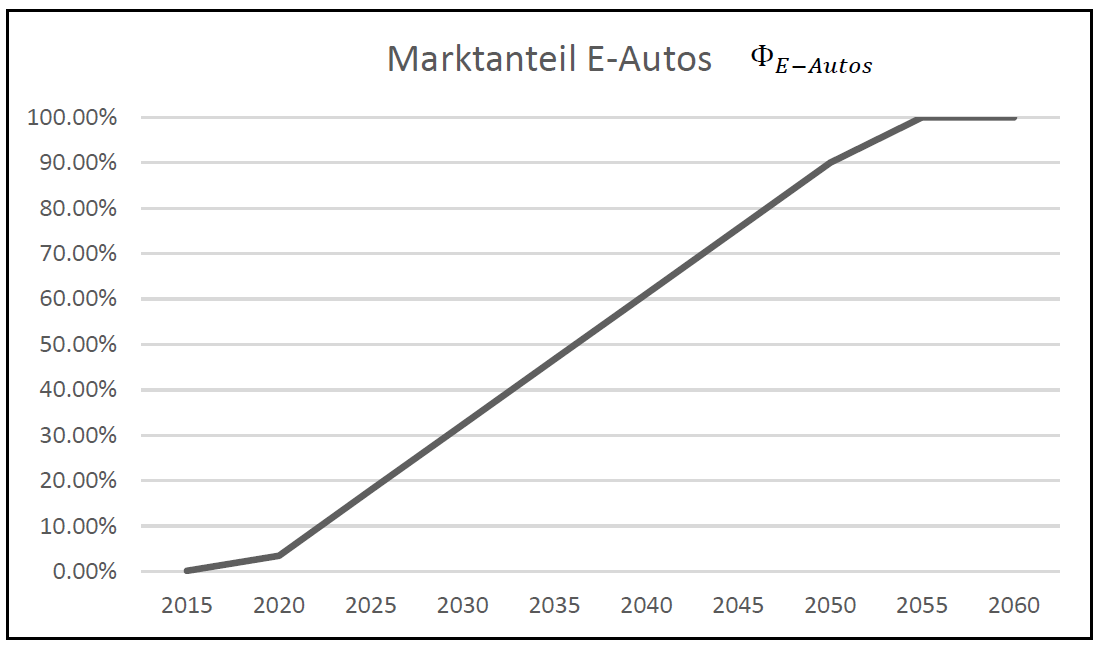
\includegraphics[width=.6\textwidth]{figures/f-04-04-01-MarktanteilE-Auto}
	\caption[Marktanteil E-Autos]{Marktanteil der E-Autos am Strassenfahrzeugbestand}
	\label{img:Marktanteil}
\end{figure}

\pagebreak


\subsection*{Unfallkosten}
\label{subsec:Unfall}

Die totalen Unfallkosten $K_{A}$, welche von der Öffentlichkeit für den betrachteten Zeitraum getragen werden müssen, werden gemäss Formel \ref{eq.10} berechnet. So ergibt sich aus der Multiplikation der Anzahl Fahrzeuge und der Unfallwahrscheinlichkeit, die Anzahl Unfälle auf der Infrastruktur. Die Anzahl Unfälle multipliziert man, um die gesamten Unfallkosten zu ermittelt, mit den Einheitskosten der jeweiligen Unfalltypen.

In Betracht gezogen werden drei verschiedene Unfalltypen [$a$,$b$,$c$].
Unfälle mit entstandenen Sachschäden und leichtverletzten Personen werden in die Kategorie $a$ eingeteilt. Für Unfälle mit schwerverletzten Beteiligten wird die Kategorie $b$ definiert und für Unfälle mit Todesfolge die Kategorie $c$. 
Die Kategorien unterscheiden sich in der Unfallhäufigkeit nach Fahrzeugart \( \gamma_{j,n} \), sowie der entstehenden Einheitskosten pro Unfall $EK_{j,n}$.

\begin{equation}
K_{A} = \sum_{t=0}^T \Biggl[ \sum_{j=1}^2 \Bigl( \sum_{n=a}^c \ EK_{j,n} \cdot \gamma_{j,n} \Bigr) \cdot DTV_{j} \cdot s_j \cdot 365 \Biggr] 
\label{eq.10}
\end{equation}

\begin{align*}
      n &=
      \begin{cases}
        \begin{aligned}
          & a  \\
          & b \\
          & c
        \end{aligned} &
        \begin{aligned}
         & \text{für}\ \thinspace \\
         & \text{für}\ \thinspace \\
         & \text{für}\ \thinspace
        \end{aligned}
        \begin{aligned}
          & {Sachsch"aden\,und\,Leichtverletzte} \\
          & {Schwerverletzte} \\
          & {Todesfall}
        \end{aligned}
      \end{cases}  \\
\end{align*}

{\setstretch{0.6}
wobei:
\begin{conditions}
 K_{A}	 		 &  Totale Unfallkosten \\
 EK_{j,n} 		 &  Einheitskosten pro Unfall nach Fahrzeugtyp \\
 DTV_{j,t}    	 &  Tägliches Verkehrsaufkommen nach Fahrzeugtyp im Jahr $t$  \\
 \gamma_{j,n} 	 &  Unfallwahrscheinlichkeit nach Fahrzeugtyp \\
 n 				 &  Unfallart  \\
\end{conditions}
} 

Wichtig anzumerken ist, dass die ermittelten Unfallrisiken die Anzahl Unfälle eines Unfalltyps pro Personenkilometer darstellen. Das bedeutet, dass für die Berechnung der Personenkilometer des MIV, der durchschnittliche Auslastungsgrad in Betracht gezogen werden muss. Somit wird in der Berechnung der Unfallkosten der $DTV_{MIV}$ mit einem Faktor 1.6 multipliziert. (\cite{Mikrozensus2015})

Die Gefahrenlage auf der Infrastruktur wird durch die Berechnung der Unfallrisiken anhand der gesamtschweizerischen Unfalldaten, abgeschätzt. Die effektive Gefahrensituation wird dadurch jedoch nicht berücksichtig. Um diese berücksichtigen zu können, müssten die Unfalldaten der Brunnenstrasse verwendet werden. Diese sind jedoch unvollständig und daher verwende ich zur Berechnung der Unfallrisiken die Unfalldaten für die ganze Schweiz. 

Da die Entwicklung der Verkehrssicherheit von verschiedensten Faktoren abhängig ist, habe ich mich im Rahmen dieser Untersuchungen aus Zeitgründen dazu entschieden, die Entwicklung der Unfallrisiken über den betrachteten Zeithorizont nicht zu variieren. 
Eine Untersuchung des Effekts der Veränderung der Unfallrisiken in Abhängigkeit der gebauten Variante erfolgt im Abschnitt \ref{subsec:Sensitivitätsanalyse}.


\subsubsection*{Unfallrisiko}
\label{subsubsec:Unfallrisiko}


Die Wahrscheinlichkeit, im Strassenverkehr einen Unfall zu erleiden, ist von verschiedenen Faktoren abhängig. In dem ich die Anzahl Unfälle nach Unfallart durch die totale Anzahl gefahrener Personenkilometer nach Fahrzeugart teile, erhalte ich das Risiko eines Unfalls pro gefahrenem Personenkilometer \( \gamma_{j,n} \). 

Unter dem Stichpunkt MIV zusammengefasst sind die Personenwagen und Motorräder sowie Motorfahrräder und schnelle E-Bikes. Die Gesamtleistung der Personenwagen in der Schweiz, lag im Jahr 2018 bei 96.9 Mrd. Personenkilometer. Die Verkehrsleistung der Motorräder, inklusive Motorfahrräder und schnelle E-Bikes lag bei 2.2 Mrd. Personenkilometer. Daraus ergibt sich eine Verkehrsleistung des MIV von 99.1 Mrd. Personenkilometer für das Jahr 2018. \\
Im Jahr 2018 erlagen insgesamt 116 Personen den Folgen eines Unfalls mit Beteiligung des MIV, 1898 Personen wurden schwer- und 12'106 Personen leicht verletzt. \\ (\cite{Verkehrsleistung2019}) (\cite{Unfall2019}) 

Das Unfallrisiko des Langsamverkehrs, den ich unter dem Begriff \textit{Velo} zusammenfasse, berechne ich nach demselben Vorgehen.
Die Verkehrsleistung der Velofahrer und langsamen E-Bikes lag im Jahr 2018 bei 2'520 Mio. Personenkilometer. \\
Im Jahr 2018 verunfallten in Zusammenhang mit dem Langsamverkehr 26 Personen tödlich. Im selben Zeitraum wurden 878 Personen schwer- und 2815 Personen leicht verletzt. \\ (\cite{Verkehrsleistung2019}) (\cite{Unfall2019})

Die berechneten Risiken sind in Tabelle \ref{tab:t-06-01-Unfallrisiko} für die verschiedenen Fahrzeuge $j$ und Unfalltypen $n$ zusammengefasst.

%=============================================================================
% Thesis Template in LaTex
%
% File:  t-05-01-IsingModel.tex -- Table for the Ising
% Author(s): Juergen Hackl <hackl@ibi.baug.ethz.ch>
%            Clemens Kielhauser <kielhauser@ibi.baug.ethz.ch>
%
% Creation:  27 Jan 2014
% Time-stamp: <Tue 2013-08-13 20:14 juergen>
%
% Copyright (c) 2014 Infrastructure Management Group (IMG)
%               http://ibi.ethz.ch
%
% More information on LaTeX: http://www.latex-project.org/
%=============================================================================

\begin{table}[hbt!]
\center
%\small\renewcommand{\arraystretch}{1.2} 
%
%
\begin{tabular}{@{}p{2.6cm} p{3.3cm} p{3.3cm} p{3.3cm}@{}} \\   
\toprule
\textbf{Fahrezugtyp\textsubscript{k}} & \textbf{Unfalltyp\,a} & \textbf{Unfalltyp\,b} & \textbf{Unfalltyp\,c} \\
\midrule
MIV      & \(1.317\,\mathrm{10^{-6}}\) $\frac{Unf"alle}{Pkm}$ & \(9.116\,\mathrm{10^{-8}}\) $\frac{Unf"alle}{Pkm}$ & \(4.7243\,\mathrm{10^{-9}}\) $\frac{Unf"alle}{Pkm}$ \\
Velo	 & \(3.818\,\mathrm{10^{-6}}\)  $\frac{Unf"alle}{Pkm}$ & \(2.643\,\mathrm{10^{-7}}\)  $\frac{Unf"alle}{Pkm}$ & \(1.37\,\mathrm{10^{-8}}\)  $\frac{Unf"alle}{Pkm}$  \\

\bottomrule

\end{tabular}
\caption[Tabelle der Unfallrisiken]{Tabelle der Unfallrisiken $\gamma_{k,n}\,\Bigl[\frac{Unf"alle_{k,n}}{Pkm_{k}}\Bigl]$}
\label{tab:t-06-01-Unfallrisiko}
\end{table}


%=============================================================================
% EOF
%

%%% Local Variables:
%%% mode: latex
%%% TeX-master: "../guidelines"
%%% End:




Nach der ausführlichen Betrachtung verschiedenster Literaturen zum Thema: \textit{Kosten die durch Strassenverkehrsunfälle entstehen} und einem Gespräch mit Herr Dr. Martani, habe ich für die Berechnung der Unfallkosten im Rahmen dieser Untersuchung die folgenden Einheitskosten der verschiedenen Unfalltypen festgelegt.

\paragraph{Kategorie $a$} Die Einheitskosten pro Unfall der Kategorie $a$ setzen sich aus den entstandenen Sachschäden und den Arbeits- und Materialkosten der Reparatur eines Fahrzeugs zusammen. Das durchschnittliche Alter eines Personenwagens in der Schweiz liegt bei 8.5 Jahren und der durchschnittliche Wert eines solchen Fahrzeuge liegt gemäss TCS bei 15'000 CHF. Die Kosten der Behandlung leichtverletzter Personen wird in dieser Betrachtung, aufgrund ihrer geringen Grösse vernachlässigt, weshalb die pro Unfall entstehenden Kosten der Kategorie $a$ mit 15'000 CHF/Unfall angesetzt, werden.

\paragraph{Kategorie $b$} Die Kosten die aufgrund eines Unfalls der Kategorie $b$ entstehen, werden durch die anfallenden Behandlungskosten der verunfallten Person bestimmt. Die Kosten durch den Erwerbsausfall für die Dauer der Arbeitsunfähigkeit, sowie die Kosten der entstandenen Sachschäden, werden in dieser Berechnung aufgrund ihrer im Vergleich zu den Behandlungskosten geringen Grösse, vernachlässigt. Die durchschnittlichen Kosten, die durch die Behandlung einer schwerverletzten Person entstehen, werden mit 110'000 $CHF/Unfall$ angesetzt. Dies entspricht 3\% der Kosten einer tödlich verunfallten Person.

\paragraph{Kategorie $c$} Diese Kosten, für einen Unfall mit Todesfolge, basieren auf der Schätzung des Werts eines statistischen Lebens. Hierfür werden gemäss dem ASTRA 3.7 Mio. $CHF/Unfall$ angesetzt.

%=============================================================================
% Thesis Template in LaTex
%
% File:  t-05-01-IsingModel.tex -- Table for the Ising
% Author(s): Juergen Hackl <hackl@ibi.baug.ethz.ch>
%            Clemens Kielhauser <kielhauser@ibi.baug.ethz.ch>
%
% Creation:  27 Jan 2014
% Time-stamp: <Tue 2013-08-13 20:14 juergen>
%
% Copyright (c) 2014 Infrastructure Management Group (IMG)
%               http://ibi.ethz.ch
%
% More information on LaTeX: http://www.latex-project.org/
%=============================================================================

\begin{table}[h!]
%\center
\flushleft
\renewcommand{\arraystretch}{1.4}
%\captionsetup{justification=centering}

\begin{tabular}{ @{} l|c @{} }
            			& Unfallkosten   $\frac{CHF}{Unfall}$	       \\ \hline
Kategorie $a$	    	&       15'000          		                \\
Kategorie $b$           &      	110'000						      \\
Kategorie $c$		    &        3.7 Mio.  		                       
\end{tabular}
\caption{Übersicht der Unfallkosten}
\label{tab:t-04-03-04-Unfallkosten}
\end{table}

%\begin{table}[h!]
%\flushleft
%\renewcommand{\arraystretch}{1.4}
%\small\renewcommand{\arraystretch}{1.2} 
%
%
%\begin{tabular}{@{}p{3.3cm} p{4cm} p{1cm} r l @{}} \\   
%\toprule
%\textbf{Interessensgruppe} & \textbf{Kostentyp} & \textbf{Symbol} & \multicolumn{2}{c}{\textbf{Einheitskosten}} 			\\
%\midrule

%\bottomrule

%\end{tabular}

%\end{table}


%=============================================================================
% EOF
%

%%% Local Variables:
%%% mode: latex
%%% TeX-master: "../guidelines"
%%% End:



\newpage




% ===========================================================================
% EOF
%

%%% Local Variables:
%%% mode: latex
%%% TeX-master: "../main"
%%% End:
